\documentclass{article}
\usepackage{graphicx}
\usepackage{subfigure}
\usepackage{longtable}
\usepackage{latexsym}
\usepackage{amsmath}
\usepackage{inputenc}
\usepackage{subfig}
\usepackage{amssymb}
\usepackage{geometry}
\usepackage{minipage-marginpar}
\begin{document}	
\title{Rapid Prototyping computer System Report}
\author{Wanjun Xu, Wenjia Liu, Anjie Wang, Hanxiang Ren}
\date{\today}
\maketitle

\newpage

\tableofcontents

\newpage

\section{Function Requirements}

\subsection{Challenge}
 The Children’s School at CMU challenged the Rapid Design and Prototyping for Computer systems class to: 
\begin{itemize}
	\item Help track the locations and activities of all members of the school 
	\item Help make dismissal an easier and less stressful process 
\end{itemize}

The whole class discussed together and had a vision scenario. According to the Human Computer Interaction Group, we have known the functions we need to implement and the other requirements we have to complete for connections with other group.

\subsection{Functional Requirements}
\subsubsection{Client Requirements}
\begin{enumerate}
	\item Show the information to the parents and the teachers
	\item Provide user control, for example: log in/out
	\item Provide message service, send and receive message or notification between teachers and parents 
	\item Show the result of data analysis, or the graph of data visualization
	\item Provide a list of children need to be dismissed to teachers.
\end{enumerate}

\subsubsection{Implementation Requirements}
Our group member compared the mainstream database, programming language, server and decided the ones which suit the situation most. 

\begin{enumerate}
	\item Read and send data from database
	\item Provide API to Data Visualization Group to show the result
\end{enumerate}


\section{Feature Comparison}
Our group member compared the mainstream database, programming language, server and decided the ones which suit the situation most. 
\subsection{Database}

\begin{table}[htbp]
\centering
  \begin{tabular}{|l|l|p{2cm}|p{2cm}|p{2cm}|p{2cm}|}
  \hline
   Database & Cost & Platform & Company & Language & Character\\
    \hline
   SQLite & Free & Windows, Linux, Unix & D. RichardHipp & Tcl, C\#, PHP, Java & Small, Fast\\
    \hline

   MySQL & Free & Windows, Linux, Unix & MySQL AB & PHP, Perl, Python & Open source, Small, Mediocre online support \\
       \hline

   Oracle & Expensive & Windows, Linux, Unix & Oracle & &\\   
       \hline
	SQL Server & \$931 & Windows, Linux, Unix & Microsoft & XML & Safe, Efficient, Smart, Big \\
	\hline
     \end{tabular}
  \caption{Database Comparison}
\end{table}

SQLite is very small and fast .So it is very good for a mobile phone. Besides ,SQLite can be applied to WEB and APP ,which others can’t. Finally we choose SQLite.

\subsection{Programming Language}
Each of us have different skills. So we divide the work into PC, APP and website. We use C\# to make a executable program in PC ,use Java to make APP and use HTML, css, JavaScript to make the website.

\begin{table}[htbp]
\centering
  \begin{tabular}{|l|p{2cm}|p{2cm}|p{2cm}|p{2cm}|}
  \hline
   Language(Framework) & MVC Framework & Testing Framework & Security Framework & Licence\\
    \hline
   C++(CppCMS) & Yes & No & Yes & MIT\\
    \hline

   Spring & Yes & Mock Objects, Unit tests & Spring Security & Apache 2.0\\
       \hline

   Python(Django) & Yes & Yes & Yes & BSD \\   
	\hline
     \end{tabular}
  \caption{Programming Language Comparison}
\end{table}

\subsection{Server}
Cloud Server is maintained by professional team, thus has better Security. However, a PC owned by child school can bear almost all of the tasks and it's free. So we select Local server, since it could fulfill our demands, and is much cheaper.

\begin{table}[htbp]
\centering
\begin{tabular}{|l|l|l|l|}
	\hline
	Server Type & Price & Storage & Security \& Stability \\
	\hline
	Local Server & ¥15k(New Server)/Free(PC) & Local Hard Disk & Fair \\
	\hline
	Cloud Server & ¥22.50/M & ¥0.24/GB/M & High \\
	\hline
	
\end{tabular}
	\caption{Server Comparison}
\end{table}

\section{Various Ends}
We designed various ends to fulfill different demand. Below are their introduction, respectively.
\subsection{Android}

 App provides different entry for different user, Parent and teacher has different interface and different authority limit. For example, parents only have access to information of their own kids, while teacher can monitor any child in his/her class (possibly the whole school).
 
\begin{figure*}[htbp]
	\centering
	\begin{minipage}[t]{0.30\linewidth}
		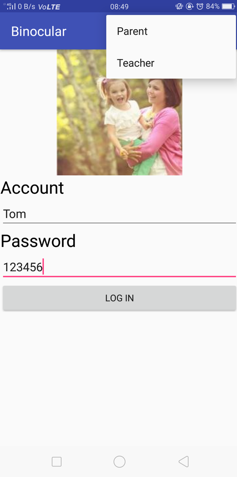
\includegraphics{img/Picture1}
	\end{minipage}
	\begin{minipage}[t]{0.30\linewidth}
		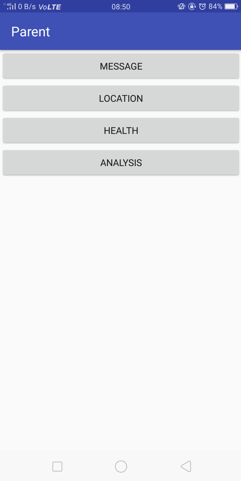
\includegraphics{img/Picture2}
	\end{minipage}
	\begin{minipage}[t]{0.30\linewidth}
		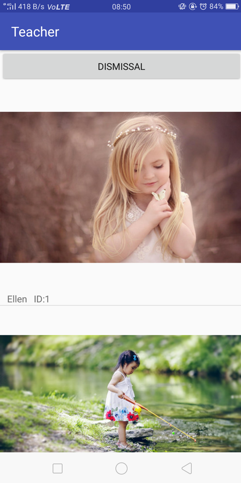
\includegraphics{img/Picture3}
	\end{minipage}	
	\caption{Different Interfaces}
\end{figure*}

\subsection{Parent Interface Breakdown}
\begin{figure*}[htbp]
	\centering
	\begin{minipage}[t]{0.30\linewidth}
		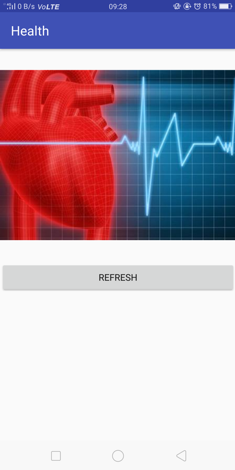
\includegraphics{img/Picture4}
	\end{minipage}
	\begin{minipage}[t]{0.30\linewidth}
		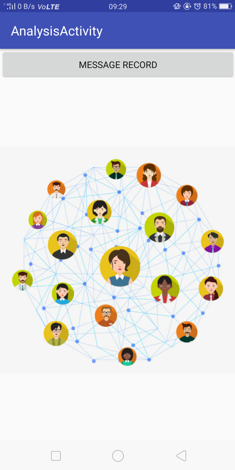
\includegraphics{img/Picture5}
	\end{minipage}
	\begin{minipage}[t]{0.30\linewidth}
		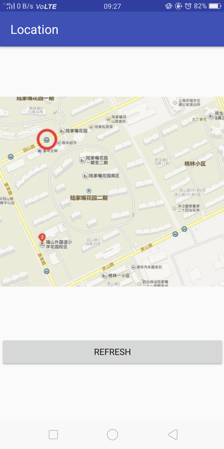
\includegraphics{img/Picture6}
	\end{minipage}	
	\caption{Different Interfaces}
\end{figure*}

\section{Individual Contribution}

\section{Lessons Learned}
\end{document}